% !TeX root = ../wireless_networks.tex
% !TeX spellcheck = en_US

\chapter{Mobile Network Layer}

\section{Mobile IP}
Mobile IP is an IETF standard communications protocol that is designed to allow mobile device users to move from one network to another while maintaining a permanent IP address.

The Mobile IP allows for location-independent routing of IP datagrams on the Internet. Each mobile node is identified by its home address disregarding its current location on the Internet. Mobile IP specifies how a mobile node registers with its home agent and how the home agent routes datagrams to the mobile node through the tunnel.

\subsection{Goals}
\begin{itemize}
\item \textbf{Goal}: Use of mobile computer on the internet.
	\item \textbf{Problem}: As soon as mobile device leaves home network and reconnect at another place, it does not receive a single packet.
	\item \textbf{Reason}: Due to routing mechanisms used on the internet.
\end{itemize}

A host sends an IP packet with the header containing a destination address with other fields. The destination address not only determines the receiver of the packet, but also the physical subnet of the receiver. 

For example, the destination address \texttt{27.36.36.69} shows that the receiver must be connected to the physical subnet with the network prefix \texttt{27.36.36}. 
\begin{itemize}
	\item Routers on the internet now look at the destination addresses of incoming packets and forward them according to internal look-up tables. 
	\item To avoid an explosion of routing tables, only prefixes are stored and further optimizations are applied. 
	\item As long as the receiver can be reached within its physical subnet, it gets the packets; as soon as it moves outside the subnet, a packet will not reach it. 
	\item A host needs a so-called \textbf{topologically correct address}.
\end{itemize}
	
	
\subsection{Assumptions}
This protocol assumes that mobile nodes will generally not change their point of attachment to the Internet more frequently than once per second.

This protocol assumes that IP unicast datagrams are routed based on the destination address in the datagram header (and not, for example,
by source address).
\subsubsection*{Quick `Solutions'}
\begin{itemize}
	\item Assign a new topologically correct IP address to the computer using \gls{dhcp}.
	\item Using dynamic DNS an update of the mapping logical name — IP address is possible.
	\item Using DNS to dynamically adapting the IP address with regard to the current location.
	\item Creation of specific routes to the mobile node.
\end{itemize}
 
\subsubsection*{Problems}
\begin{itemize}
	\item Moving to a new location assigns new IP address which nobody knows and it is almost impossible to find a mobile host on the internet which has just changed its address.
	\item \gls{dns} needs some time before it updates the internal tables necessary to map a logical name to an IP address. This approach does not work if the mobile node moves quite often. The internet and DNS have not been built for frequent updates.
\end{itemize}

There is a severe problem with higher layer protocols like \gls{tcp} which rely on IP addresses. Changing the IP address while still having a \gls{tcp} connection open
means breaking the connection. A \gls{tcp} connection is identified by the tuple (source IP address, source port, destination IP address, destination port), also
known as a \textbf{socket pair} (a socket consists of address and port). Therefore, a \gls{tcp} connection cannot survive any address change. Breaking \gls{tcp} connections is not an
option, using even simple programs like telnet would be impossible. The mobile node would also have to notify all communication partners about the new address.

\subsection{Requirements}
Since the \textit{quick solutions} obviously did not work, a more general architecture had to be designed. Many field trials and proprietary systems finally led to mobile IP as a standard to enable mobility on the internet. Several requirements accompanied the development of the standard:


\subsubsection{Compatibility}
\begin{itemize}
	\item A new standard cannot introduce changes to existing network protocols.
	\item People do not want to change their applications just for mobility.
	\item Mobile has to work with current operating systems.
	\item Mobile IP must not require special media or \gls{mac}/LLC protocols.
	\item Mobile IP has to ensure that users can still access all the other servers and systems	on the internet.
\end{itemize}

\subsubsection{Transparency}

\begin{itemize}
	\item Mobility should remain \textit{invisible} for many higher layer protocols and applications.  
	\item Higher layers should continue to work even if	the mobile computer has changed its point of attachment to the network.
\end{itemize}


\subsubsection{Scalability and Efficiency}
\begin{itemize}
\item Introducing a new mechanism to the internet must not jeopardize its efficiency. 
	\item Enhancing IP for mobility must not generate too many new messages flooding the whole network.
	\item Special care has to be taken considering the lower bandwidth of wireless links.
	\item It is crucial for a mobile IP to be scalable over a large number of participants in the whole internet, worldwide.
\end{itemize}

\subsubsection{Security}
\begin{itemize}
	\item Mobility poses many security problems.
	\item The minimum requirement is that of all the messages related to the management of Mobile IP are authenticated. 
	\item The IP layer must be sure that if it forwards a packet to a mobile host that this host receives the packet.
	\item The IP layer can only guarantee that the IP address of the receiver is correct.
	\item There are no ways of preventing fake IP addresses or other attacks.
\end{itemize}


The goal of a mobile IP can be summarized as: \emph{supporting end-system mobility while maintaining scalability, efficiency, and compatibility in all respects with existing applications and Internet protocols}.


\subsection{Entities and Terminology}
Mobile IP introduces the following entities and terms. Figure \ref{fig:mobile_ip_example}
illustrates an example scenario.

%%%%%%%%%%%%%%%%%%%%%%%%%%%%%
%							%
%		FIGURE				%
%							%
%%%%%%%%%%%%%%%%%%%%%%%%%%%%%

\begin{figure}[ht!]
	\centering
	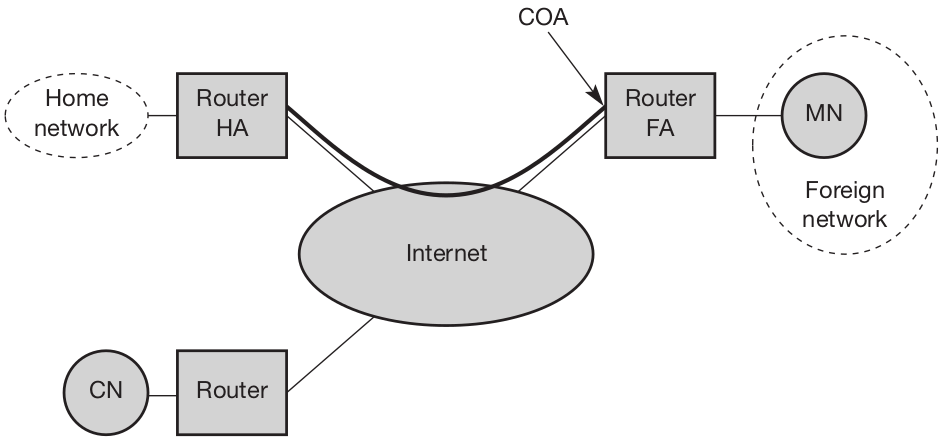
\includegraphics[width=0.7\textwidth]{mobile-ip-example-network}
	\caption{Mobile IP example network}\label{fig:mobile_ip_example}
\end{figure}


\subsection*{Entities}

\subsubsection[Mobile Node]{Mobile Node (MN)}
\begin{itemize}
	\item Is an end-system or router that can change its point of attachment to the internet using mobile IP. 
	\item The MN keeps its IP address and can continuously communicate with any other system on the internet as long as link-layer connectivity is given.
	\item MNs are not necessarily small devices such as laptops with antennas or mobile phones; a router onboard an aircraft can be a powerful mobile node.
\end{itemize}

\subsubsection[Home Agent]{Home Agent (HA)}
\begin{itemize}
	\item The \gls{ha} provides several services for the MN and is located in the home network.
	\item The tunnel for packets toward the MN starts at the \gls{ha}.
	\item The \gls{ha} maintains a location registry, i.\ e.\, it is informed of the MN's location by the current \gls{coa}. 
	\item Three alternatives for the implementation of an \gls{ha} exist:
	\begin{itemize}
			\item On a router that is responsible for the home network.
			\item On an arbitrary node in the subnet.
			\item On the \textit{router} but this time only acting as a manager for MNs belonging to a virtual home network. 
	\end{itemize}
\end{itemize}


\subsubsection[Foreign Agent]{Foreign Agent (FA)}
\begin{itemize}
	\item The \gls{fa} can provide several services to the MN during its visit to the foreign network. 
	\item The \gls{fa} can have the \gls{coa}, acting as tunnel endpoint and forwarding packets to the MN. 
	\item The \gls{fa} can be the default router for the MN. 
	\item \gls{fa}s can also provide security services because they belong to the foreign network as opposed to the MN which is only visiting.
	\item For mobile IP functioning, \gls{fa}s are not necessarily needed. 
	\item Typically, an \gls{fa} is implemented on a router for the subnet the MN attaches to.
\end{itemize}

\subsection*{Terminology}

\subsubsection[Correspondent Node]{Correspondent Node (CN)}
\begin{itemize}
	\item A peer with which a mobile node is communicating.  
	\item A \gls{cn} may be either mobile or stationary.
\end{itemize}

\subsubsection{Home Network}
\begin{itemize}
	\item The home network is the subnet the MN belongs to with respect to its IP address. 
	\item No mobile IP support is needed within the home network.
\end{itemize}

\subsubsection{Foreign Network}
Any network other than the MN's Home Network.

\subsubsection{Home Address}
\begin{itemize}
	\item An IP address that is assigned for an extended period of time to an MN.
	\item It remains unchanged regardless of where the node is attached to the Internet.
\end{itemize}

\subsubsection[Care-of-address]{Care-of-address (COA)}
\begin{itemize}
	\item The COA defines the current location of the MN from an IP point of view. 
	\item All IP packets sent to the MN are delivered to the
	\gls{coa}, not directly to the IP address of the MN. 
	\item Packet delivery toward the MN is done using a tunnel.
	\item There are two different possibilities for the location of the COA:
	
	\begin{itemize}
		\item \textbf{Foreign Agent \gls{coa}}: The \gls{coa} could be located at the \gls{fa}, i.\ e.\, the \gls{coa} is an IP address of the \gls{fa}. The \gls{fa} is the tunnel end-point and forwards packets to the MN.
		\item \textbf{Co-located \gls{coa}}: The \gls{coa} is co-located if the MN temporarily acquired an additional IP address which acts as \gls{coa}. 
	\end{itemize}
\end{itemize}


The example network in Figure \ref{fig:mobile_ip_example} shows the following situation: 
\begin{itemize}
	\item A \gls{cn} is connected via a router to the internet, as are the home network and the foreign network. 
	\item The \gls{ha} is implemented on the router connecting the home network with the internet, an \gls{fa} is implemented on the router to the foreign network.
	\item The MN is currently in the foreign network. 
	\item The tunnel for packets toward the MN starts at the \gls{ha} and ends at the \gls{fa}, for the \gls{fa} has the \gls{coa} in this example.
\end{itemize}


\subsection{IP Packet Delivery}
Figure \ref{fig:packet_delivery_mobile} illustrates packet delivery to and from the MN using the example network of Figure \ref{fig:mobile_ip_example}. 
\begin{steps}
	\item A correspondent node \gls{cn} wants to send an IP packet to the MN. \gls{cn} does not need to know anything about the MN’s current location and sends the packet as usual to the IP address of MN. This means that \gls{cn} sends an IP packet with MN as a destination address and \gls{cn} as a source address. \label{stp:step1}
	\item The \gls{ha} now intercepts the packet. The packet is encapsulated and tunneled to the \gls{coa}. A new header is put in front of the old IP header showing the \gls{coa} as new destination and \gls{ha} as source of the encapsulated packet. \label{stp:step2}
	\item The foreign agent now decapsulates the packet, i.\ e.\ , removes the additional header, and forwards the original packet with \gls{cn} as source and MN as destination to the MN.\label{stp:step3}
	\item The MN sends the packet as usual with its own fixed IP address as source and \gls{cn}'s address as destination.\label{stp:step4}
\end{steps}

The router with the \gls{fa} acts as default router and forwards the packet in the same way as it would do for any other node in the foreign network. As long as \gls{cn} is a fixed node the remainder is in the fixed internet as usual. If \gls{cn} were also a mobile node residing in a foreign network, the same mechanisms as described in \ref{stp:step1} through \ref{stp:step3} would apply now in the other direction.
%%%%%%%%%%%%%%%%%%%%%%%%%%%%%
%							%
%		FIGURE				%
%							%
%%%%%%%%%%%%%%%%%%%%%%%%%%%%%
	
\begin{figure}[hpt]
	\centering
	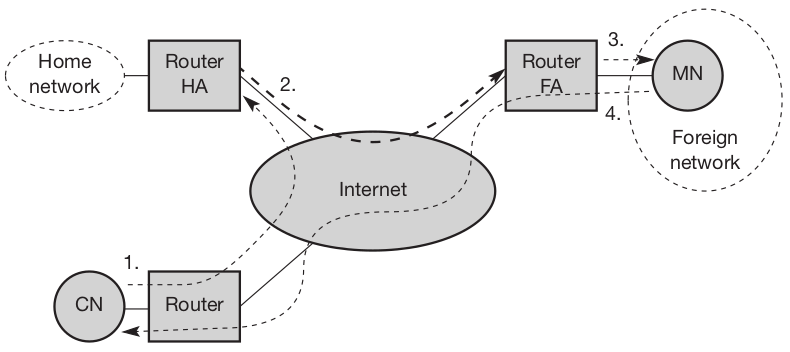
\includegraphics[width=0.8\textwidth]{packet-delivery-mobile}
	\caption{Packet delivery to and from the mobile node}\label{fig:packet_delivery_mobile}
\end{figure}


\subsection*{Working of Mobile IP}
Mobile IP has two addresses for a mobile host: \textit{one home address} and \textit{one care-of address}. 

\begin{itemize}
	\item The home address is permanent; the care-of addresses changes as the mobile host moves from one network to another. 
	\item To make the change of address transparent to the rest of the Internet requires a home agent and a foreign agent. 
	\item The specific function of an agent is performed in the application layer. 
	\item When the mobile host and the foreign agent are the same, the care-of address is called a co-located care-of address. 
	\item To communicate with a remote host, a mobile host goes through three phases:
	\begin{enumerate}
		\item agent discovery, 
		\item registration, and 
		\item data transfer.
	\end{enumerate}
	 
\end{itemize}


\subsection{Agent Discovery}
One initial problem of an MN after moving is how to find a foreign agent. How does the MN discover that it has moved? For this purpose mobile IP describes two methods: 

\begin{itemize}
\item \textit{agent advertisement} and 
\item \textit{agent solicitation},
\end{itemize}
which are in fact router discovery methods plus extensions.

\subsubsection{Agent Advertisement}
For the first method, foreign agents and home agents advertise their presence periodically using special agent \textit{advertisement messages}. These advertisement messages can be seen as a beacon broadcast into the subnet. For these advertisements \gls{icmp} messages are used with some mobility extensions. Routers in the fixed network implementing this standard also advertise their routing service periodically to the attached links.

%%%%%%%%%%%%%%%%%%%%%%%%%%%%%
%							%
%		FIGURE				%
%							%
%%%%%%%%%%%%%%%%%%%%%%%%%%%%%
	
	\begin{figure}[ht!]
	\centering
	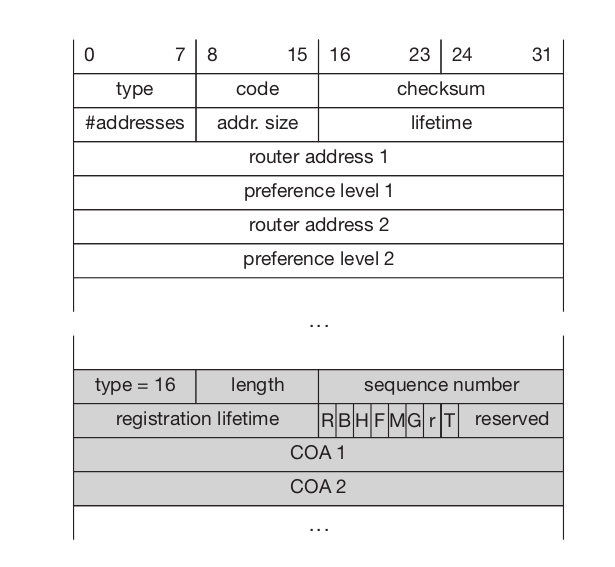
\includegraphics[width=0.8\textwidth]{agent-advertisement-packet}
	\caption[Agent advertisement packet.]{Agent advertisement packet (RFC 1256 + mobility extension)}\label{fig:agent_advertisement}
	\end{figure}
	
	
The agent advertisement packet with the extension for mobility is shown in Figure \ref{fig:agent_advertisement}. 
\begin{itemize}
	\item The upper part represents the \textit{\gls{icmp} packet}.
	\item The lower part is the \textit{extension needed for mobility}.
\end{itemize}
 The fields necessary on lower layers for the agent advertisement are not shown in this figure. Clearly, mobile nodes must be reached with the appropriate link layer address. The TTL field of the IP packet is set to 1 for all advertisements to avoid forwarding them.

The IP destination address according to standard router advertisements can be either set to \verb|224.0.0.1|, which is the multicast address for all systems on a link, or to the broadcast address \verb|255.255.255.255|.

The fields in the \gls{icmp} part are defined as follows. 

\begin{multicols}{2}
\begin{enumerate}
	\item The \textbf{type} is set to 9.
	
	\item the \textbf{code} can be 0, if the agent also routes traffic from non-mobile nodes, or 16, if it does not route anything other than mobile traffic.
	
	\item \textbf{Lifetime} denotes the length of time this advertisement is valid.
	
	\item Foreign agents are at least required to forward packets from the mobile node. The number of addresses advertised with this packet is in \textbf{\#addresses}.
	
	\item \textbf{Preference} levels for each address help a node to choose the router that is the most eager one to get a new node.
\end{enumerate}
\end{multicols}



The difference compared with standard ICMP advertisements is what happens after the router addresses. This extension for mobility has the following
fields defined:

\begin{multicols}{2}
	\begin{enumerate}
		\item \textbf{type} is set to 16.
		
		\item \textbf{length} depends on the number of COAs provided with the message and equals $ 6 + 4*(number of addresses) $.
		
		\item An agent shows the total number of advertisements sent since initialization in the \textbf{sequence number}.
		
		\item By the \textbf{registration lifetime} the agent can specify the maximum lifetime in seconds a node can request during registration.
	\end{enumerate}
\end{multicols}


The following bits specify the characteristics of an agent in detail.
	
	\begin{multicols}{2}
			\begin{enumerate}
			\item The \textbf{R} bit (registration) shows, if a registration with this agent is required even when using a co-located COA at the MN
			
			\item If the agent is currently too busy to accept new registrations it can set the \textbf{B} bit
			
			\item The following two bits denote if the agent offers services as a home agent \textbf{(H)} or foreign agent \textbf{(F)} on the link where the advertisement has been sent.
			
			\item Bits \textbf{M} and \textbf{G} specify the method of encapsulation used for the tunnel.
			
			\item \textbf{M} can specify minimal encapsulation and \textbf{G} generic routing encapsulation.
			
			\item In the first version of mobile IP the \textbf{V} bit specified the use of header compression
			
			\item Now the field \textbf{r} at the same bit position is set to zero and must be ignored.
			
			\item The new field \textbf{T} indicates that reverse tunneling is supported by the FA.
		\end{enumerate}
	\end{multicols}


The following fields contain the \textbf{COAs} advertised:
\begin{itemize}
\item A foreign agent setting the F bit must advertise at least one COA.
\end{itemize}

A mobile node in a subnet can now receive agent advertisements from either its home agent or a foreign agent. This is one way for the MN to discover its location.

\subsubsection{Agent Solicitation}
\begin{itemize}
\item If no agent advertisements are present or the inter-arrival time is too high, and an MN has not received a \gls{coa} by other means, e.\ g.\, \gls{dhcp}, the mobile node must send \textbf{agent solicitations}. 

\item Care must be taken to ensure that these solicitation messages do not flood the network, but basically an MN can search for an \gls{fa} endlessly sending out solicitation messages

\item Typically, a mobile node can send out three solicitations, one per second, as soon as it enters a new network.

\item If a node does not receive an answer to its solicitations it must decrease the rate of solicitations exponentially to avoid flooding the network until it reaches a maximum interval between solicitations.


\item Discovering a new agent can be done anytime, not just if the MN is not connected to one.

\item After these steps of advertisements or solicitations the MN can now receive a \gls{coa}, either one for an \gls{fa} or a co-located \gls{coa}. 

\item The MN knows its location (home network or foreign network) and the capabilities of the agent.

\item The next step for the MN is the registration with the \gls{ha} if the MN is in a foreign network.
\end{itemize}


\subsection{Registration}
Having received a COA, the MN has to register with the HA. The main purpose of the registration is to inform the HA of the current location for correct forwarding of packets. Registration can be done in two different ways depending on the location of the COA.

\subsubsection[COA at FA]{COA at The FA}
If the COA is at the FA, registration is done as illustrated in Figure \ref{fig:mobile_node_registration} (left).

\begin{itemize}
	\item The MN sends its registration request containing the COA (see Figure \ref{fig:registration-request}) to the FA which is forwarding the request to the HA.
	\item The HA now sets up a \textbf{mobility binding} containing the mobile node’s home IP address and the current COA. 
	\item Additionally, the mobility binding contains the lifetime of the registration which is negotiated during the registration process. 
	\item Registration expires automatically after the lifetime and is deleted; so, an MN should re-register before expiration. 
	\item This mechanism is necessary to avoid mobility	bindings which are no longer used. 
	\item After setting up the mobility binding, the HA sends a reply message back to the FA which forwards it to the MN.
\end{itemize}


\subsubsection[Co-located COA]{COA is Co-located}
If the COA is co-located, registration can be simpler, as shown in Figure \ref{fig:mobile_node_registration} (right).
\begin{itemize}
	\item The MN may send the request directly to the HA and vice versa.
	\item This is also the registration procedure for MNs returning to their home network. 
	\item Here, they also register directly with the HA. 
	\item However, if the MN received an agent advertisement from the FA it should register via	this FA if the \textbf{R} bit is set in the advertisement.
\end{itemize}

%%%%%%%%%%%%%%%%%%%%%%%%%%%%%
%							%
%		FIGURE				%
%							%
%%%%%%%%%%%%%%%%%%%%%%%%%%%%%

\begin{figure}[hb!]
	\centering
	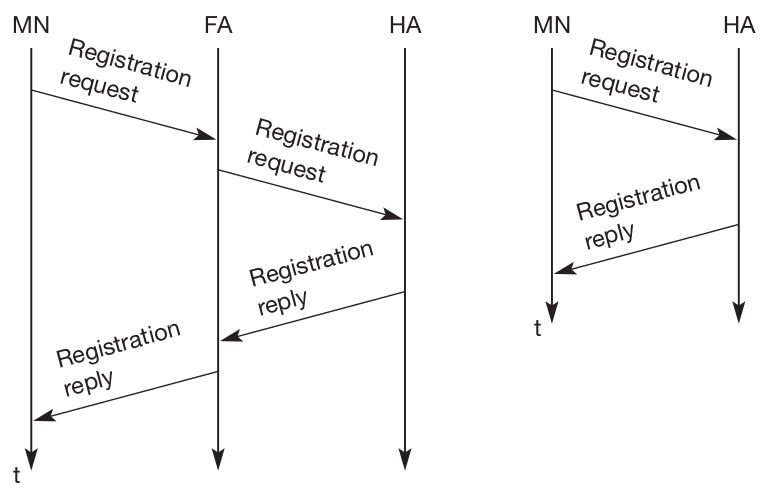
\includegraphics[width=0.8\textwidth]{mobile-node-registration}
	\caption{Registration of a mobile node via the FA or directly with the HA}\label{fig:mobile_node_registration}
\end{figure}



\subsubsection*{Registration Request}
UDP packets are used for \textbf{registration requests}. The IP source address of the packet is set to the interface address of the MN, the IP destination address is that of the FA or HA (depending on the location of the COA). The UDP destination port is set to 434. UDP is used because of low overheads and better performance
compared to \gls{tcp} in wireless environments. The fields relevant for mobile IP registration requests follow as UDP data (see Figure \ref{fig:registration-reply}). The fields are defined as follows.


This allows for simultaneous bindings. The following bits denote the requested behavior for packet forwarding.

%%%%%%%%%%%%%%%%%%%%%%%%%%%%%
%							%
%		FIGURE				%
%							%
%%%%%%%%%%%%%%%%%%%%%%%%%%%%%

\begin{figure}[pht]
	\centering
	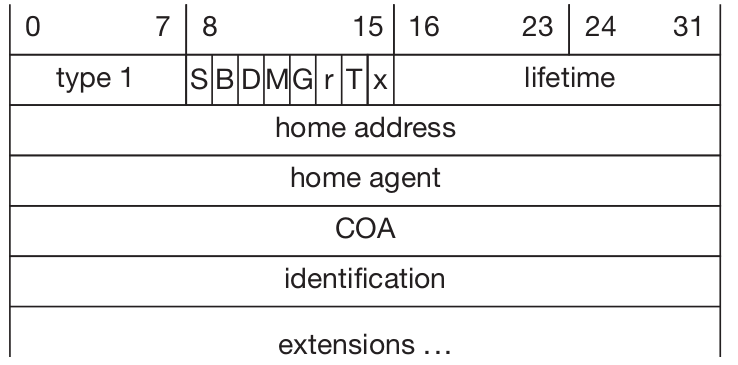
\includegraphics[width=0.8\textwidth]{registration-request}
	\caption{Registration request}\label{fig:registration-request}
\end{figure}

\begin{multicols}{2}
\begin{enumerate}
	\item The first field type is set to 1 for a registration request
	
	\item With the \textbf{S} bit an MN can specify if it wants the HA to retain prior mobility bindings
	
	\item Setting the B bit generally indicates that an MN also wants to receive the broadcast packets which have been received by the HA in the home
	network
	
	\item If an MN uses a co-located COA, it also takes care of the decapsulation at the tunnel endpoint. The \textbf{D} bit indicates this behavior
	
	\item \textbf{M} and \textbf{G} denote the use of minimal encapsulation or generic routing encapsulation, respectively
	
	\item \textbf{T} indicates reverse tunneling
	
	\item \textbf{r} and \textbf{x} are set to zero
	
	\item \textbf{lifetime} denotes the validity of the registration in seconds
	
	\item A value of zero indicates de-registration; all bits set indicates infinity
	
	\item The \textbf{home address} is the fixed IP address of the MN
	
	\item \textbf{home agent} is the IP address of the HA, and COA represents the tunnel endpoint
	
	\item The 64 bit \textbf{identification} is generated by the MN to identify a request and match it with registration replies. This field is used for protection against replay attacks of registrations.
	
	\item The extensions must at least contain parameters for authentication
\end{enumerate}
\end{multicols}


\subsubsection*{Registration Reply}

%%%%%%%%%%%%%%%%%%%%%%%%%%%%%
%							%
%		FIGURE				%
%							%
%%%%%%%%%%%%%%%%%%%%%%%%%%%%%
	
	\begin{figure}[hb!]
	\centering
	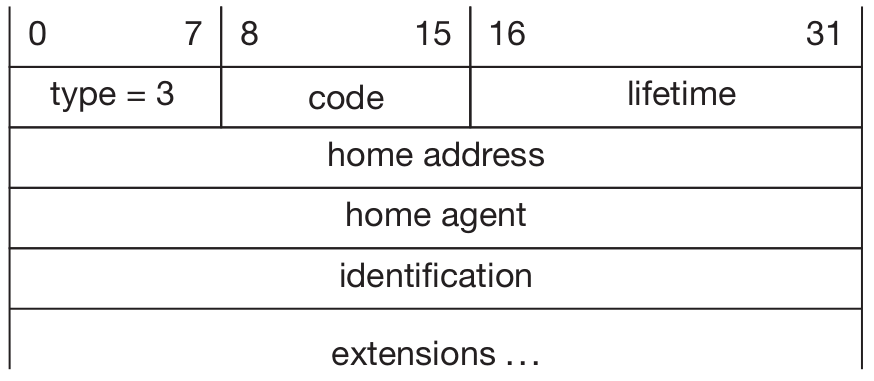
\includegraphics[width=0.8\textwidth]{registration-reply}
	\caption{Registration reply}\label{fig:registration-reply}
	\end{figure}
	
A \textbf{registration reply}, which is conveyed in a UDP packet, contains:
\begin{multicols}{2}
\begin{enumerate}
	\item a \textbf{type} field set to 3 and
	
	\item a \textbf{code} indicating the result of the registration request.
	
	\item \textbf{lifetime} field indicates how many seconds the registration is valid if it was successful.
	
	\item \textbf{home address} and \textbf{home agent} are the addresses of the MN and the HA, respectively.
	
	\item 64-bit \textbf{identification} is used to match registration requests with replies. The value is based on the identification field from the registration and the authentication method.
	
	\item \textbf{extensions} must at least contain parameters for authentication.
	
\end{enumerate}
\end{multicols}

\subsection{Tunneling and Encapsulation}
The following describes the mechanisms used for forwarding packets between the HA and the COA, as shown in Figure \ref{fig:packet_delivery_mobile} \ref{stp:step2} (\textnp{Figure \ref{fig:packet_delivery_mobile} काे \ref{stp:step2} मा Tunneling र Encapsulation को कुरा बताइएको छ।}). 

%%%%%%%%%%%%%%%%%%%%%%%%%%%%%
%							%
%		FIGURE				%
%							%
%%%%%%%%%%%%%%%%%%%%%%%%%%%%%

\begin{figure}[hpt]
	\centering
	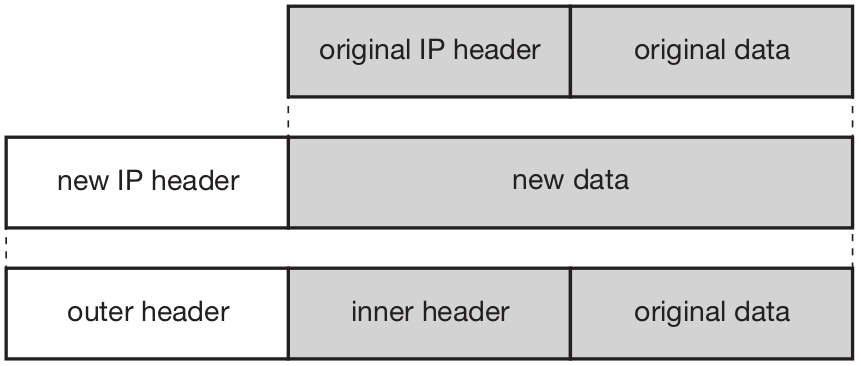
\includegraphics[width=0.7\textwidth]{ip-encapsulation}
	\caption{IP encapsulation}\label{fig:ip_encapsulation}
\end{figure}
%--------------------------------------------------------------------

\subsubsection*{Tunnel}
\begin{multicols}{2}
	\begin{itemize}
		\item A \textbf{tunnel} establishes a virtual pipe for data packets between a tunnel entry and a tunnel endpoint. 
		\item Packets entering a tunnel are forwarded inside the tunnel and leave the tunnel unchanged. 
		\item Tunneling, i.\ e.\ , sending a packet through a tunnel, is achieved by using encapsulation.
	\end{itemize}
\end{multicols}


\subsubsection*{Encapsulation}
\begin{multicols}{2}
\begin{itemize}
	\item \textbf{Encapsulation} is the mechanism of taking a packet consisting of packet header and data and putting it into the data part of a new packet. 
	\item The reverse operation, taking a packet out of the data part of another packet, is called \textbf{decapsulation}. 
	\item Encapsulation and decapsulation are the operations typically performed when a packet is transferred from a higher protocol layer to a lower layer or from a lower to a higher layer respectively. 
	\item Here, these functions are used within the same layer.
\end{itemize}

\end{multicols}


This mechanism is shown in Figure {\ref{fig:ip_encapsulation}} and describes exactly what the HA at the tunnel entry does. 
\begin{multicols}{2}
	\begin{itemize}
		\item The HA takes the original packet with the MN as destination, puts it into the data part of a new packet and sets the new IP header in such a way that the packet is routed to the COA. 
		\item The new header is also called the \textbf{outer header}. 
		\item Additionally, there is an \textbf{inner header} which can be identical to the original header as this is the case for IP-in-IP encapsulation, or the inner header can be computed during encapsulation.
	\end{itemize}
\end{multicols}


\subsubsection{IP-in-IP Encapsulation}
There are different ways of performing the encapsulation needed for the tunnel between HA and COA. Mandatory for mobile IP is \textbf{IP-in-IP encapsulation}. Figure \ref{fig:ip_ip_encapsulation} shows a packet inside the tunnel.

%%%%%%%%%%%%%%%%%%%%%%%%%%%%%
%							%
%		FIGURE				%
%							%
%%%%%%%%%%%%%%%%%%%%%%%%%%%%%

\begin{figure}[hb!]
	\centering
	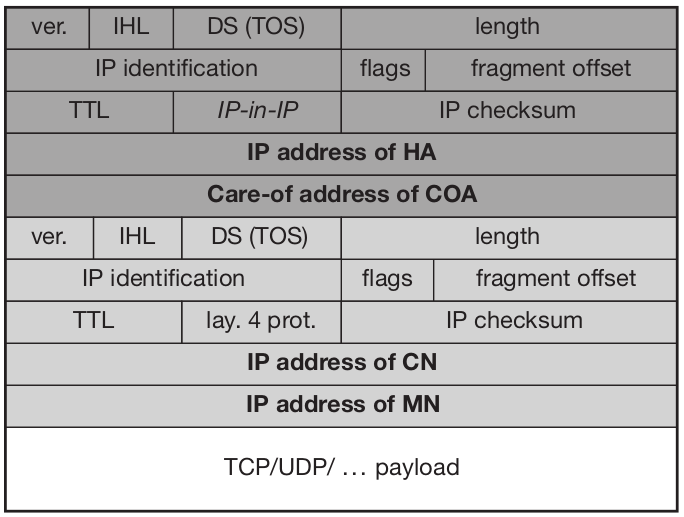
\includegraphics[width=0.8\textwidth]{ip-in-ip-encapsulation}
	\caption{IP-in-IP encapsulation}\label{fig:ip_ip_encapsulation}
\end{figure}


The fields of the outer header are set as follows:
\begin{multicols}{2}
	\begin{itemize}
	\item The version field \textbf{ver} is 4 for IP version 4, the internet header length (IHL) denotes the length of the outer header in 32 bit words.
	
	\item \textbf{DS (TOS)} is just copied from the inner header
	
	\item the \textbf{length} field covers the complete encapsulated packet.
	
	\item TTL have no special meaning for mobile IP.
	
	\item \textbf{TTL} must be high enough so the packet can reach the tunnel endpoint.
	
	\item field, \textbf{IP-in-IP}, is the type of the protocol used in the IP payload. This field is set to 4, the protocol type for IPv4 because again an IPv4 packet follows after this outer header.
	
	\item IP \textbf{checksum} is calculated as usual.
	
	\item the \textbf{IP address of the HA} is the tunnel entry as source address.
	
	\item \textbf{the COA} is the tunnel exit point as destination address
\end{itemize}
\end{multicols}

	
If no options follow the outer header, the inner header starts with the same fields as just explained. This header remains almost unchanged during encapsulation, thus showing the original sender CN and the receiver MN of the packet.

The only change is TTL which is decremented by 1. This means that the whole tunnel is considered a single hop from the original packet’s point of view. This is a very important feature of tunneling as it allows the MN to behave as if it were attached to the home network. No matter how many real hops the packet has to take in the tunnel, it is just one (logical) hop away for the MN. Finally, the payload follows the two headers.



\subsubsection{Minimal encapsulation}


As seen with IP-in-IP encapsulation, several fields are redundant. For example, TOS is just copied, fragmentation is often not needed etc.  \textbf{Minimal encapsulation} (shown in Figure \ref{fig:minimal-encapsulation}) is an optional encapsulation method for mobile IP. 
\begin{multicols}{2}
	\begin{itemize}
		\item The tunnel entry point and endpoint are specified. 
		\item In this case, the field for the type of the following header contains the value 55 for the minimal encapsulation protocol. 
		\item The inner header is different	for minimal encapsulation. 
		\item The type of the following protocol and the address of the MN are needed. 
		\item If the \textbf{S} bit is set, the original sender address of the CN is included as omitting the source is quite often not an option. 
		\item No field for fragmentation offset is left in the inner header and minimal encapsulation does not work with already fragmented packets.
	\end{itemize}
\end{multicols}

%%%%%%%%%%%%%%%%%%%%%%%%%%%%%
%							%
%		FIGURE				%
%							%
%%%%%%%%%%%%%%%%%%%%%%%%%%%%%

\begin{figure}[ht!]
	\centering
	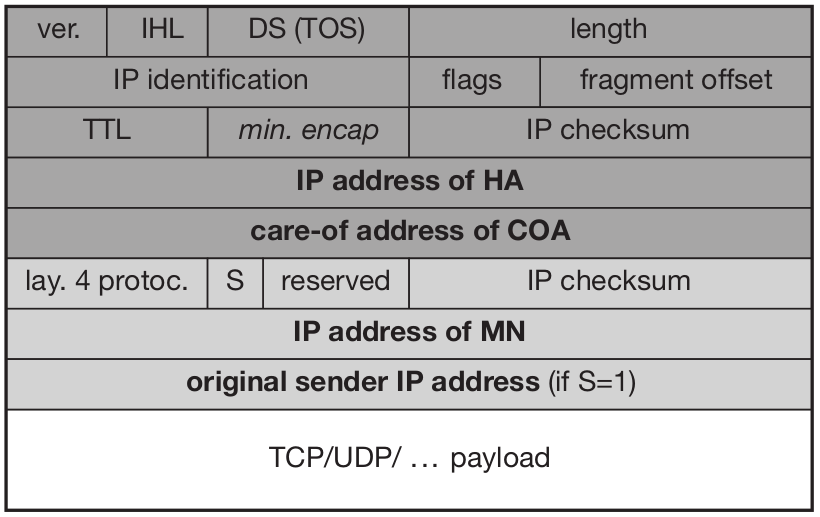
\includegraphics[width=0.8\textwidth]{minimal-encapsulation} 
	\caption{Minimal encapsulation}
	\label{fig:minimal-encapsulation}
\end{figure}

\subsubsection{Generic Routing Encapsulation}
While IP-in-IP encapsulation and minimal encapsulation work only for IP, the encapsulation scheme also supports other network layer protocols in addition to IP. \textbf{Generic routing encapsulation (GRE)} allows the encapsulation of packets of one protocol suite into the payload portion of a packet of another
protocol suite. Figure \ref{fig:generic-routing-encapsulation} shows this procedure. 

%%%%%%%%%%%%%%%%%%%%%%%%%%%%%
%							%
%		FIGURE				%
%							%
%%%%%%%%%%%%%%%%%%%%%%%%%%%%%

\begin{figure}[hb!]
	\centering
	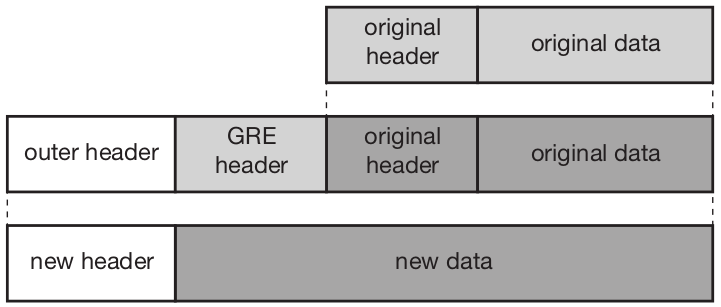
\includegraphics[width=0.8\textwidth]{generic-routing-encapsulation}
	\caption{Generic routing encapsulation}\label{fig:generic-routing-encapsulation}
\end{figure}

\begin{itemize}
	\item The packet of one protocol suite with the original packet header and data is taken and a new GRE header is prepended. 
	\item Together this forms the new data part of the new	packet. 
	\item Finally, the header of the second protocol suite is put in front.
\end{itemize}


\ref{fig:protocol-fields-for-gre} shows on the left side the fields of a packet inside the tunnel
between home agent and COA using GRE as an encapsulation scheme. The outer header is the standard IP header with HA as source
address and COA as destination address. The protocol type used in this outer IP header is 47 for GRE. The other fields of the outer packet, such as TTL and TOS,
may be copied from the original IP header. However, the TTL must be decremented by 1 when the packet is decapsulated to prevent indefinite forwarding.

%%%%%%%%%%%%%%%%%%%%%%%%%%%%%
%							%
%		FIGURE				%
%							%
%%%%%%%%%%%%%%%%%%%%%%%%%%%%%
	
	\begin{figure}[ht!]
	\centering
	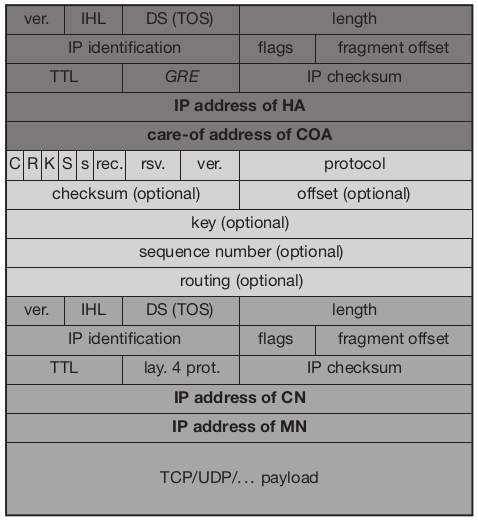
\includegraphics[width=0.8\textwidth]{protocol-fields-for-gre}
	\caption{Protocol fields for GRE}\label{fig:protocol-fields-for-gre}
	\end{figure}
	
The GRE header starts with several flags indicating if certain fields are pre sent or not. A minimal GRE header uses only 4 bytes; nevertheless, GRE is
flexible enough to include several mechanisms in its header. The C bit indicates
if the checksum field is present and contains valid information. 
\begin{multicols}{2}
	\begin{itemize}
		\item If \textbf{C} is set, the	\textbf{checksum} field contains a valid IP checksum of the GRE header and the payload. 
		\item The \textbf{R} bit indicates if the offset and routing fields are present and contain	valid information.
		\item The \textbf{offset} represents the offset in bytes for the first source \textbf{routing} entry. 
		\item The routing field, if present, has a variable length and contains fields for source routing.
		\item \textbf{key} field may be used for authentication. If this field is present, the \textbf{K} bit is set.
		\item The \textbf{sequence} number bit \textbf{S} indicates if the sequence number field is present, if the s bit is set, strict source routing is used. 
		\item The \textbf{recursion control} field (\textbf{rec.}) distinguishes GRE from IP-in-IP and minimal encapsulation. 
		\item The \textbf{reserved} fields must be zero and are ignored on reception. 
		\item The \textbf{version} field contains 0 for the GRE version. 
		\item The 2 byte \textbf{protocol} field represents the protocol of the packet following the GRE header. 
	\end{itemize}
\end{multicols}

	
Figure \ref{fig:protocol-fields-for-gre-rfc-2784} shows the simplified header of GRE, which is a more generalized version of GRE.

This version does not address mutual encapsulation and ignores several protocol-specific nuances on purpose. 

\begin{multicols}{2}
	\begin{itemize}
		\item The field \textbf{C} indicates if a checksum is present. 
		\item The next 5 bits are set to zero, then 7 reserved bits follow. 
		\item The \textbf{version} field contains the value zero. 
		\item The protocol type, defines the protocol of the payload. 
		\item If the flag C is set,	then \textbf{checksum} field and a field called \textbf{reserved1} follows. 
		\item The reserved1 field is constant zero set to zero follow.
	\end{itemize}
\end{multicols}

%%%%%%%%%%%%%%%%%%%%%%%%%%%%%
%							%
%		FIGURE				%
%							%
%%%%%%%%%%%%%%%%%%%%%%%%%%%%%

\begin{figure}[ht!]
	\centering
	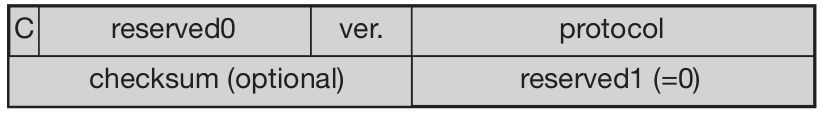
\includegraphics[width=0.8\textwidth]{gre-rfc-2784}
	\caption{Simplified header of GRE}\label{fig:protocol-fields-for-gre-rfc-2784}
\end{figure}

	
\subsection{Optimizations}
Imagine the following scenario. A Nepalese and a Chinese meet at a conference on North Korea. Both want to use their laptops for exchanging data, both run mobile IP for mobility support. Now recall Figure \ref{fig:packet_delivery_mobile} and think of the way the packets between both computers take.

\begin{itemize}
	\item If the Nepalese sends a packet to the Chinese, his computer sends the data to the HA of the Chinese, i.\ e., from North Korea to China. 
	\item The HA in China now encapsulates the packets and tunnels them to the COA of the Chinese laptop on North Korea. 
	\item This means that although the computers might be only meters away, the packets have to travel around the world! This inefficient behavior of a non-optimized mobile IP is called \textbf{triangular routing}. 
	\item The triangle is made of the three segments, CN to HA, HA to COA/MN, and MN back to CN.
\end{itemize}


%With the basic mobile IP protocol all packets to the MN have to go through the HA. This can cause unnecessary overheads for the network between CN and HA, but also between HA and COA, depending on the current location of the MN. As the example shows, latency can increase dramatically. This is particularly unfortunate if the MNs and HAs are separated by, e.g., transatlantic links.


\textbf{Triangle Routing Problem} is considered as one of the problems facing the implementation of Mobile IP. When a CN sends traffics to MN, the following sequence must be done. 
\begin{enumerate}
	\item CN sends packets to the HA.
	\item HA encapsulates these packets and tunnels	them to the FA.
	\item The FA de-tunnels the packets and delivers them to the Mobile Node. 
\end{enumerate}
This behavior is known as triangular routing. As shown in Figure \ref{fig:triangular-routing}, the route taken by these packets is triangle in nature, and the most extreme case of routing can be observed when the Correspondent Node and Mobile Node are in the same subnet.


%%%%%%%%%%%%%%%%%%%%%%%%%%%%%
%							%
%		FIGURE				%
%							%
%%%%%%%%%%%%%%%%%%%%%%%%%%%%%

\begin{figure}[ht!]
	\centering
	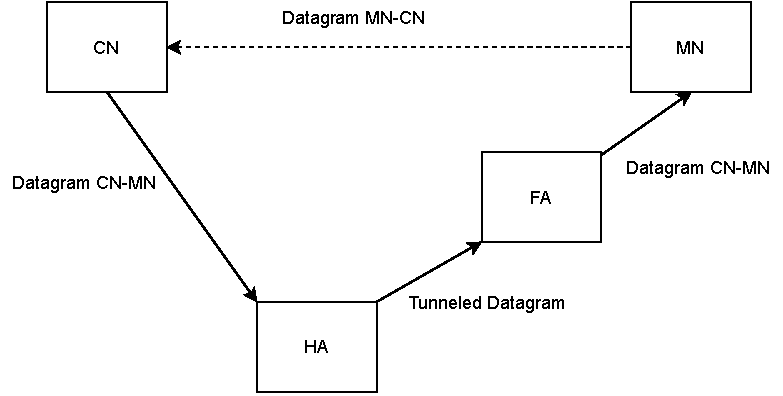
\includegraphics[width=0.8\textwidth]{triangular-routing}
	\caption{Triangular routing}\label{fig:triangular-routing}
\end{figure}

\begin{itemize}
	\item One way to optimize the route is to inform the CN of the current location of the MN. 
	\item The CN can learn the location by caching it in a \textbf{binding cache} which is a part of the local routing table for the CN. 
	\item The appropriate entity to inform the CN of the location is the HA. 
\end{itemize}

The optimized mobile IP protocol needs four additional messages.

\begin{enumerate}
\item \textbf{Binding request}: 
\begin{itemize}
	\item Any node that wants to know the current location of an MN can send a binding request to the HA. 
	\item The HA can check if the MN has allowed dissemination of its current location. 
	\item If the HA is allowed to reveal the location it sends back a binding update.
\end{itemize}

\item \textbf{Binding update}:
\begin{itemize}
	\item This message sent by the HA to CNs reveals the current location of an MN. 
	\item The message contains the fixed IP address of the MN and the COA. 
	\item The binding update can request an acknowledgment.
\end{itemize}


\item \textbf{Binding acknowledgment}: If requested, a node returns this acknowledgment after receiving a binding update message.

\item \textbf{Binding warning}: 
\begin{itemize}
	\item If a node decapsulates a packet for an MN, but it is not the current FA for this MN, this node sends a binding warning. 
	\item The warning contains MN’s home address and a target node address, i.\ e.\, the address of the node that has tried to send the packet to this MN. 
	\item The recipient of the warning then knows that the target node could benefit from obtaining a fresh binding for the MN. 
	\item The recipient can be the HA, so the HA should now send a binding update to the node that obviously has a wrong COA for the MN.
\end{itemize}

\end{enumerate}

Figure \ref{fig:foreign-agent-optimized-mobile-ip} explains these additional four messages together with the case of an MN changing its FA. 

\begin{itemize}
	\item The CN can request the current location from the HA. 
	\item If allowed by the MN, the HA returns the COA of the MN via an update message. 
	\item The CN acknowledges this update message and stores the mobility binding. 
	\item Now the CN can send its data directly to the current foreign agent $FA_{old}$. 
	\item $ FA_{old} $ forwards the packets to the MN. 
	\item This scenario shows a COA located at an FA. 
	\item Encapsulation of data for tunneling to the COA is now done by the CN, not the HA.
\end{itemize}


The MN might now change its location and register with a new foreign agent, $ FA_{new} $. This registration is also forwarded to the HA to update its location database. Furthermore, $ FA_{new} $ informs $ FA_{old} $ about the new registration of MN. MN’s registration message contains the address of $ FA_{old} $ for this purpose. Passing
this information is achieved via an update message, which is acknowledged by $ FA_{old} $. 

Without the information provided by the new FA, the old FA would not get to know anything about the new location of MN. In this case, CN does not know anything about the new location, so it still tunnels its packets for MN to the old FA, $ FA_{old} $. This FA now notices packets with destination MN, but also knows that it is not the current FA of MN. $ FA_{old} $ might now forward these packets to the new COA of MN which is $ FA_{new} $ in this example. This forwarding of packets is another optimization of the basic Mobile IP providing \textbf{smooth handovers}. 

Without this optimization, all packets in transit would be lost while the MN moves from one FA to another. % With \gls{tcp} as the higher layer protocol this would result in severe performance degradation.

%%%%%%%%%%%%%%%%%%%%%%%%%%%%%
%							%
%		FIGURE				%
%							%
%%%%%%%%%%%%%%%%%%%%%%%%%%%%%
	\begin{figure}[ht!]
	\centering
	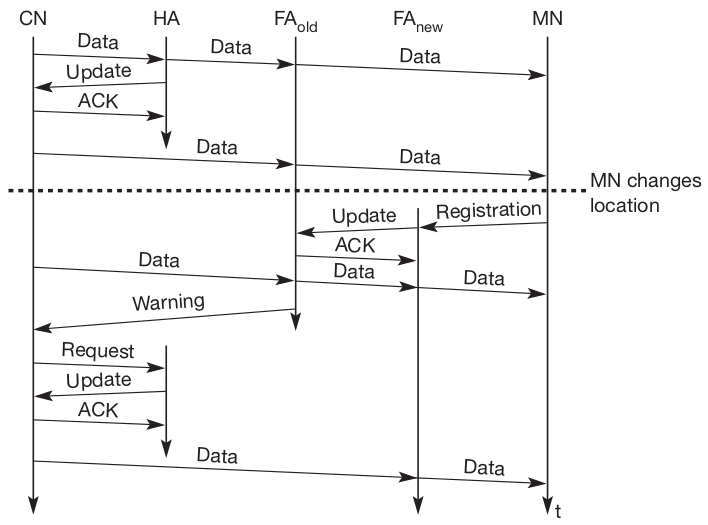
\includegraphics[width=0.8\textwidth]{foreign-agent-optimized-mobile-ip}
	\caption{Change of the foreign agent with an optimized mobile IP}\label{fig:foreign-agent-optimized-mobile-ip}
	\end{figure}

To tell CN that it has a stale binding cache:
\begin{multicols}{2}
	\begin{enumerate}
		\item $ FA_{old} $ sends, a binding warning message to CN. 
		\item CN then requests a binding update. (The warning could also be directly sent to the HA triggering an update). 
		\item The HA sends an update to inform the CN about the new location, which is acknowledged. 
		\item Now CN can send its packets directly to $ FA_{new} $, again avoiding triangular routing. 
	\end{enumerate}
\end{multicols}
	


\subsubsection*{Problems with this optimization}
\begin{multicols}{2}
\begin{itemize}
	\item Security problems such as \textit{tunnel hijacking}.
	\item All users do not want to reveal their current location to others.
\end{itemize}
\end{multicols}



\subsection[DHCP]{Dynamic Host Configuration Protocol (DHCP)}
\begin{itemize}
	\item \gls{dhcp} is an automatic configuration protocol used on IP networks. 
	\item DHCP allows a computer to join an IP-based network without having a pre-configured IP address. 
	\item DHCP is a protocol that assigns unique IP addresses to devices, then releases and renews these addresses as devices leave and re-join the network.
	\item If a new computer is connected to a network, DHCP can provide it with all the necessary information for full system integration into the network, e.\ g.\ , addresses of a DNS server and the default router, the subnet mask, the domain name, and an IP address. 
	\item Providing an IP address, makes DHCP very attractive for mobile IP as a source of care-of-addresses.
\end{itemize}

DHCP is based on a client/server model as shown in Figure \ref{fig:basic-dhcp-config}. DHCP clients send a request to a server (DHCPDISCOVER in the example) to which
the server responds. A client sends requests using MAC broadcasts to reach all devices in the LAN. A DHCP relay might be needed to forward requests across inter-working units to a DHCP server.

%%%%%%%%%%%%%%%%%%%%%%%%%%%%%
%							%
%		FIGURE				%
%							%
%%%%%%%%%%%%%%%%%%%%%%%%%%%%%
	
	\begin{figure}[hb!]
	\centering
	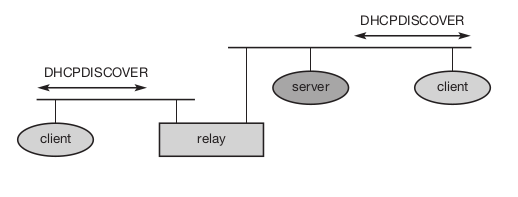
\includegraphics[width=0.8\textwidth]{basic-dhcp-config}
	\caption{Basic DHCP configuration}\label{fig:basic-dhcp-config}
	\end{figure}


A typical initialization of a DHCP client is shown in Figure \ref{fig:dhcp-client-init}. The figure shows one client and two servers. 
\begin{itemize}
	\item The client broadcasts a DHCPDISCOVER into the subnet. There might be a relay to forward this broadcast. 
	\item In the case shown, two servers receive this broadcast and determine the configuration they can offer to the client. 
	\item One example for this could be the checking of available IP addresses and choosing one for the client. 
	\item Servers reply to the client’s request with DHCPOFFER and offer a list of configuration parameters. 
	\item The client can now choose one of the configurations offered.
	\item The client in turn replies to the servers, accepting one of the configurations and rejecting the others using DHCPREQUEST.
	\item If a server receives a DHCPREQUEST with a rejection, it can free the reserved configuration for other possible clients. 
	\item The server with the configuration accepted by the client now confirms the configuration with DHCPACK. This completes the initialization phase.
	
\end{itemize}

If a client leaves a subnet, it should release the configuration received by the server using DHCPRELEASE. Now the server can free the context stored for the client and offer the configuration again. The configuration a client gets from a server is only leased for a certain amount of time, it has to be reconfirmed from time to time. Otherwise the server will free the configuration. This timeout of configuration helps in the case of crashed nodes or nodes moved away without releasing the context.

%%%%%%%%%%%%%%%%%%%%%%%%%%%%%
%							%
%		FIGURE				%
%							%
%%%%%%%%%%%%%%%%%%%%%%%%%%%%%

\begin{figure}[ht!]
	\centering
	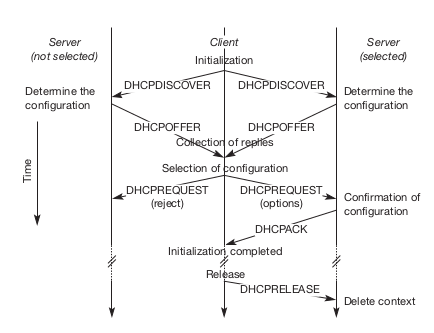
\includegraphics[width=0.8\textwidth]{dhcp-client-init}
	\caption{Client initialization via DHCP}\label{fig:dhcp-client-init}
\end{figure}

%DHCP is a good candidate for supporting the acquisition of care-of-addresses for mobile nodes. The same holds for all other parameters needed, such as addresses of the default router, DNS servers, the timeserver etc. A DHCP server should be located in the subnet of the access point of the mobile node, or at least a DHCP relay should provide forwarding of the messages. RFC 3118 specifies authentication for DHCP messages which is needed to protect mobile nodes from malicious DHCP servers. Without authentication, the mobile node cannot trust a DHCP server, and the DHCP server cannot trust the mobile node.

\subsubsection*{Advantages of DHCP}
\gls{dhcp} provides the following benefits.

\paragraph*{Reliable IP Address Configuration} 
\gls{dhcp} minimizes configuration errors caused by manual IP address configuration, such as typographical errors, or address conflicts caused by the assignment of an IP address to more than one computer at the same time.

\paragraph*{Reduced Network Administration} 
\gls{dhcp} includes the following features to reduce network administration:
\begin{itemize}
	\item Centralized and automated TCP/IP configuration.
	
	\item The ability to define TCP/IP configurations from a central location.
	
	\item The ability to assign a full range of additional TCP/IP configuration values by means of \gls{dhcp} options.
		
	\item The efficient handling of IP address changes for clients that must be updated frequently, such as those for portable devices that move to different locations on a wireless network.
		
	\item The forwarding of initial \gls{dhcp} messages by using a \gls{dhcp} relay agent, which eliminates the need for a \gls{dhcp} server on every subnet.
					
\end{itemize}

